\section{Design theory}\label{sec:trans_theory}
In this section, the reasoning behind the design of the protocol is described. That is, any thoughts and ideas, about the inner workings of the protocol, that has ether been put into code or discarded for whatever reason. This whole section is, thus, a description of what went on before the actual software implementation took place.


\subsection{Speed versus reliability}
A dilemma, when formulating how the protocol should function is, that as high as possible speeds are desired.\marginnote{Ref. to the ''project ideas'' document} On the other hand, one must remember, that we want to make it as painless as possible for the user application to use the protocol (meaning the user should be able to expect successful delivery).

A UDP\footnote{User datagram protocol.}-like protocol design would no doubt be one of the best ways to achieve a low overhead. The UDP protocol provides a connectionless service, where datagrams\footnote{The transfer unit of the UDP protocol.} are sent and then forgotten. That way the receiver does not have to spend bandwidth to acknowledge successful receptions. Additionally, the header size of a datagram is quite small, as there is no overhead used for error- or flow control. Datagrams are also sent without any way of knowing whether they are received in-order or not.

\nomenclature{UDP}{User datagram protocol}\nomenclature{TCP}{Transmission control protocol}

Using a TCP\footnote{Transmission control protocol.} inspired protocol instead would enable the transport layer to provide a much more reliable service. Now, in the TCP protocol, flow- and error control is added, as well as congestion control. Every packet is assigned a sequence number, ensuring they are passed on to the server application correctly, by the receiving transport layer protocol. Every packet is also acknowledged by the receiver, if it is successfully recorded. If not, the sender re-sends them. All these things combined makes TCP a lot more reliable, but it also increases it's header size to around three times the size of the UDP header. Especially if one is not sending a lot of data in each packet, the header can take up a large percentage of the combined (header plus data) package size.%%%%%%

Although the services provided by the data link layer guarantees an error-free connection, we cannot be sure data is received in the correct order.\marginnote{Ref.} Both because the data link layer itself does not provide \textit{that} guarantee, but also because the backbone priority system could possibly shift the order. As there is an uncertainty here, we need to establish a way to ensure that data is passed on from the protocol to the above layer in the correct order. This can be done by using a system, where each outgoing data packet is assigned a sequence number.

Sequence numbering provides a way to make sure packets are delivered in the correct order, but with just the sequence number, it is not certain that the data bytes \textit{inside} a given packet are in the correct order. For this a checksum calculation is called for.

All summed up, a protocol design, that will ensure in-order delivery of data, is needed. Features as flow- and congestion control is ignored. Mainly because the communication is going to take place via sound after all: We can safely say that the transfer speeds will not be high and congestion is unlikely to occur.\marginnote{Ref.} After all, the communication line is inherently half-duplex, making the data flow one-way (at a single point in time) by nature.

Coincidentally the RUDP\footnote{Reliable UDP protocol.} described in \cite{RUDP} suits the needs well on many points. Therefore some of the properties, portrayed in the following parts, are based on those of the RUDP. Note that the RUDP document is an \textit{internet draft}, meaning it is work-in-progress (and seemingly ot updated in a long time).

\nomenclature{RUDP}{Reliable User Datagram Protocol}


\subsection{Addressing processes}
The data link layer takes care of the node-to-node delivery, where each node has an address. There is a problem however: The receiving data link layer protocol strips the header, containing the node address, off before the information reaches the transport layer protocol. Figure \ref{fig:trans_osi_modelish} shows this: The solid lines are the actual data transmission path, while the dotted lines are the individual layers' ''pseudo-transmission paths''. \textbf{DH} is the data link layer protocol header and, as we can see, it is not passed on up through the layers.

\begin{figure}[htb]
 \centering
 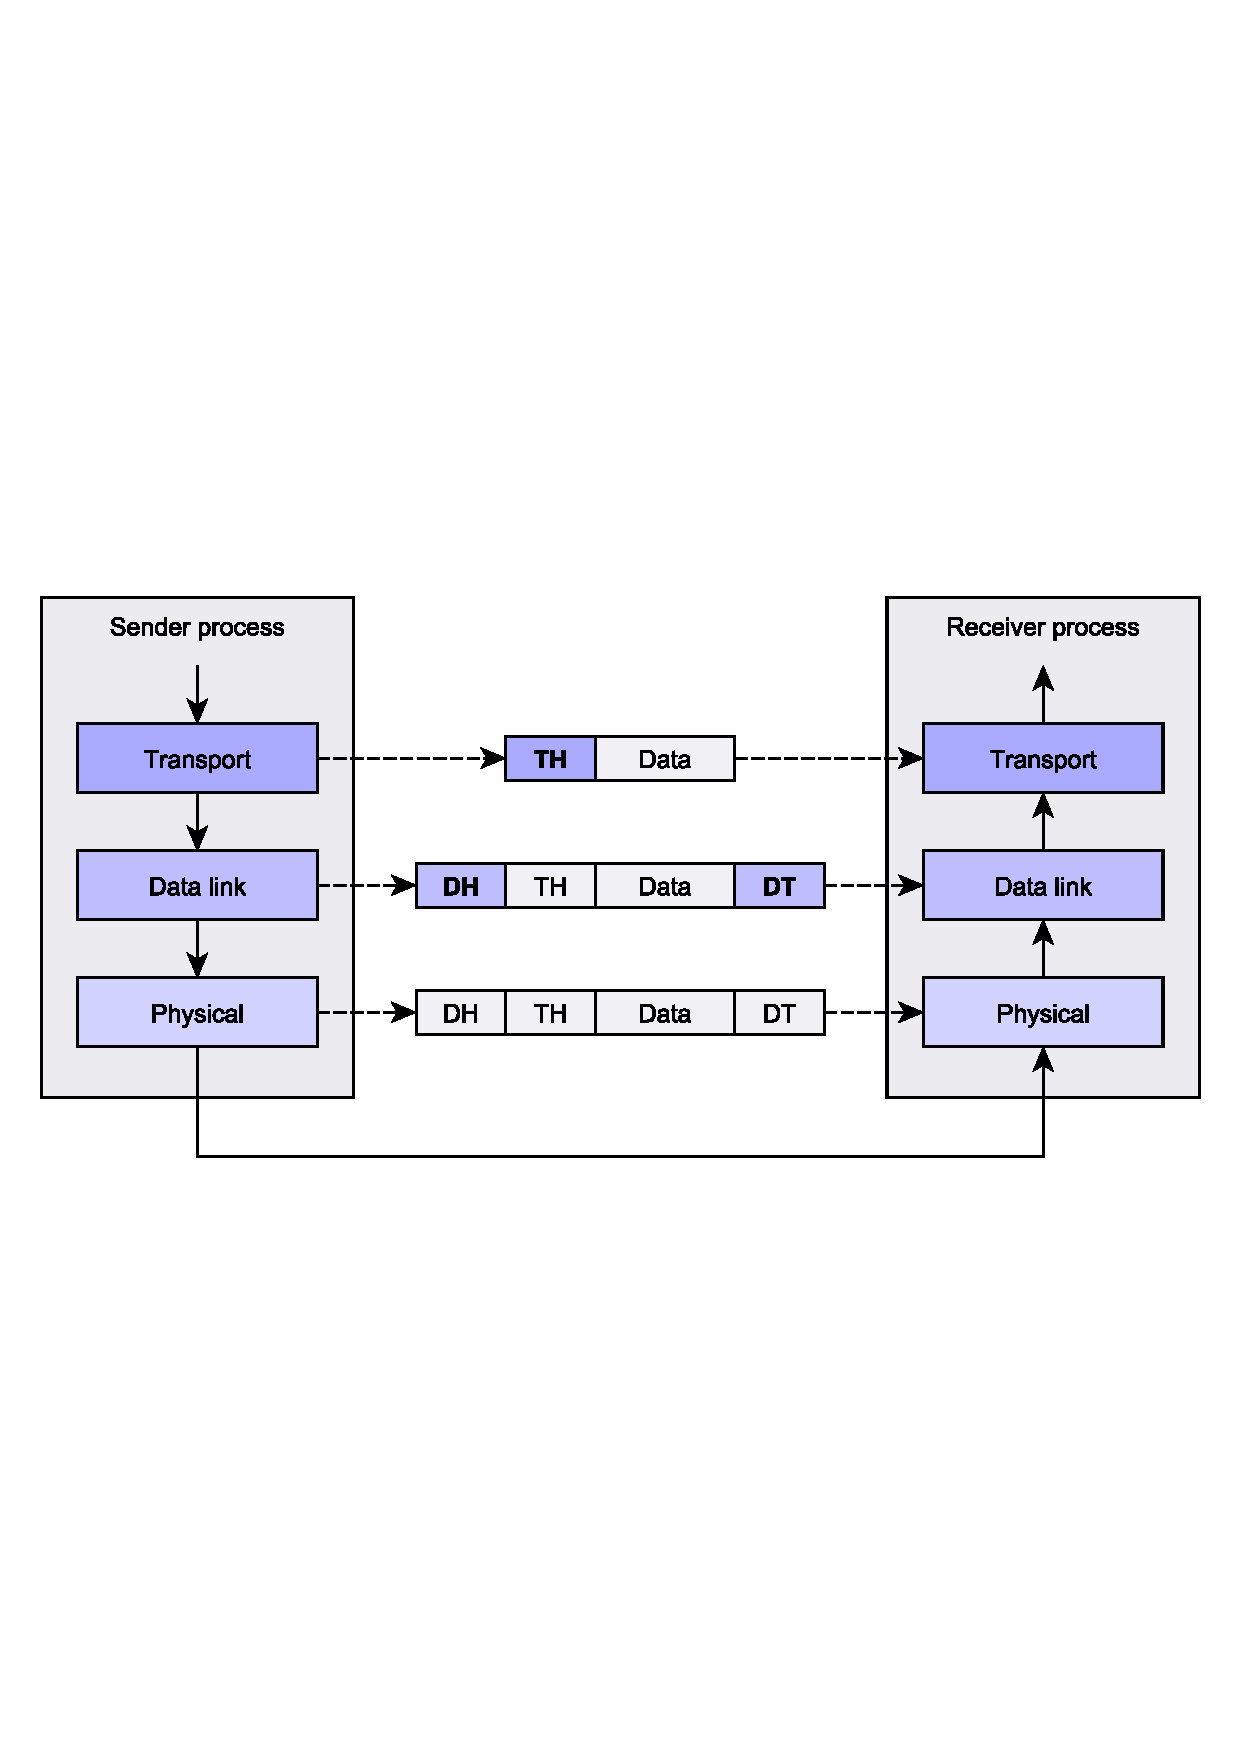
\includegraphics[scale=0.62,trim=0 267 0 267]{content/graphics/trans_osi_modelish.pdf}%trim=l b r t
 \caption{The transmission path from sending to receiving transport layer protocol}
 \label{fig:trans_osi_modelish}
\end{figure}

To obtain a way of distinguishing signaling processes from each other, another attribute must be introduced: A port number.\footnote{Port number, in this text, is separate from the port number normally associated with a process when it \textit{binds} via some kind of Internet socket. Still, the term is used, as it's purpose is the same.} The port number, assigned to a certain server application, must be known to the client before it starts sending. That is the only way the client process will know where to send data. In the protocol, we select the port number to be eight bits long. This reasoning behind this choice is, that it is unlikely that we have to server lots of applications at a time. Add to that, that we wish to keep a minimal overhead size (a higher port number would add more bits to the header), as we don't have a lot of bandwidth available to begin with.


\subsection{Packet format}
From the above layer the protocol expects to just receive a stream of data. The order in which the data is received is significant, but the data itself is not. When received, the data bytes will be packed into packets of a maximum length of 255 bytes (it can be smaller). A maximum length of 255 bytes seems like a sensible size.\marginnote{Better reasoning/reference}

All the attributes described above, leads to the packet header format as shown in Table \ref{tab:trans_packet_header}. It is 8 bytes long, which leaves a maximum possible amount of 248 bytes of data per packet. The flags field will be treated throughout the next parts of this section.

\begin{table}[htb]
 \centering
 \begin{tabular*}{0.74\textwidth}{@{\extracolsep{\fill}}|c|c|c|c|c|c|c|c|c|c|c|c|c|c|c|c|}
  %
  \multicolumn{4}{l}{\texttt{0}} & \multicolumn{4}{r}{\texttt{7}} & \multicolumn{4}{l}{\texttt{8}} & \multicolumn{4}{r}{\texttt{15}}\\
  \hline
  %
  \multicolumn{8}{|c|}{   \multirow{2}{*}{Source port addr.}   } & \multicolumn{8}{c                  |}{   \multirow{2}{*}{Destination port addr.}   }\\
  \multicolumn{8}{|c|}{                                        } & \multicolumn{8}{p{0.334\textwidth} |}{                                             }\\
  \hline                                                                           % ^ above width is to acquire symmetry
  %
  \texttt{S} & \texttt{A} & \texttt{N} & \texttt{R} & \texttt{E} & \texttt{ } & \texttt{ } & \texttt{C} & \multicolumn{8}{c|}{  \multirow{3}{*}{Total length}  }\\
  \texttt{Y} & \texttt{C} & \texttt{U} & \texttt{S} & \texttt{A} & \texttt{0} & \texttt{0} & \texttt{H} & \multicolumn{8}{c|}{                         }\\
  \texttt{N} & \texttt{K} & \texttt{L} & \texttt{T} & \texttt{K} & \texttt{ } & \texttt{ } & \texttt{K} & \multicolumn{8}{c|}{                         }\\
  \hline
  %
  \multicolumn{8}{|c|}{    \multirow{2}{*}{Sequence number}    } & \multicolumn{8}{c|}{     \multirow{2}{*}{Acknowledgment number}        }\\
  \multicolumn{8}{|c|}{                                        } & \multicolumn{8}{c|}{                                                   }\\
  \hline
  %
  \multicolumn{16}{|c|}{   \multirow{2}{*}{Checksum}   }\\
  \multicolumn{16}{|c|}{                               }\\
  \hline
  %
 \end{tabular*}
 \caption{Transport layer protocol packet header}
 \label{tab:trans_packet_header}
\end{table}


\subsection{Sequence numbering}
As mentioned, sequence numbering is introduced to make sure the receiving protocol passes on data to the above layer in the correct order. Every packet that is sent will have such a number attached. The sequence number is eight bits long. A packet will also have an eight bit acknowledgment number, which is closely related to the sequence number, as we shall see.

When a connection is initiated, a random sequence number between $0$ and $2^8-1$ is selected. This number will be attached to a so-called SYN packet (the \texttt{SYN} flag is then set), which is used to establish a connection and synchronise the senders sequence numbers with the receivers. Each party must then increment this number by 1 before sending a response packet, except in a few special cases, which will be discussed.

The acknowledgment number is also a number of 8 bits. It indicates, to the sender, the sequence number of a packet which the receiver has received correctly. If \texttt{ACK} flag is set it means the acknowledgment number is valid.

\subsection{Error control}
In order to avoid the risk of bytes shifting position inside one packet, a checksum is calculated. This checksum also serves as a strong error detection mechanism, although it should, in theory, not be needed as the data link layer protocol provides error control. The checksum type chosen is the cyclic redundancy check, or CRC, using the CRC-CCITT generator polynomial $x^{16} + x^{12} + x^5 + 1$.\marginnote{Elaborate on CRC + Ref.} This provides checksum size of 16 bits.

\nomenclature{CRC}{Cyclic redundancy check}

The header of the packet is always getting it's checksum calculated. If the \texttt{CHK} flag bit is set, a checksum is calculated for the whole package. This is the default, and preferred way, of transmission.

\subsection{Operation}
Because of the need to synchronise sequence numbers,the protocol uses \textit{handshaking} in the form of the SYN packet and the response to it. When a connection is first opened, a SYN packet, with a random sequence number attached, is sent. The receiver must then respond within a set time frame to acknowledge the connection. This response must have an acknowledgment number equal to the sequence number just received. Figure \ref{fig:trans_syn_transfer} shows the connection establishment taking place. Disconnected and connected refers to the protocols internal status: How it perceives itself.

\begin{figure}[htb]
 \centering
 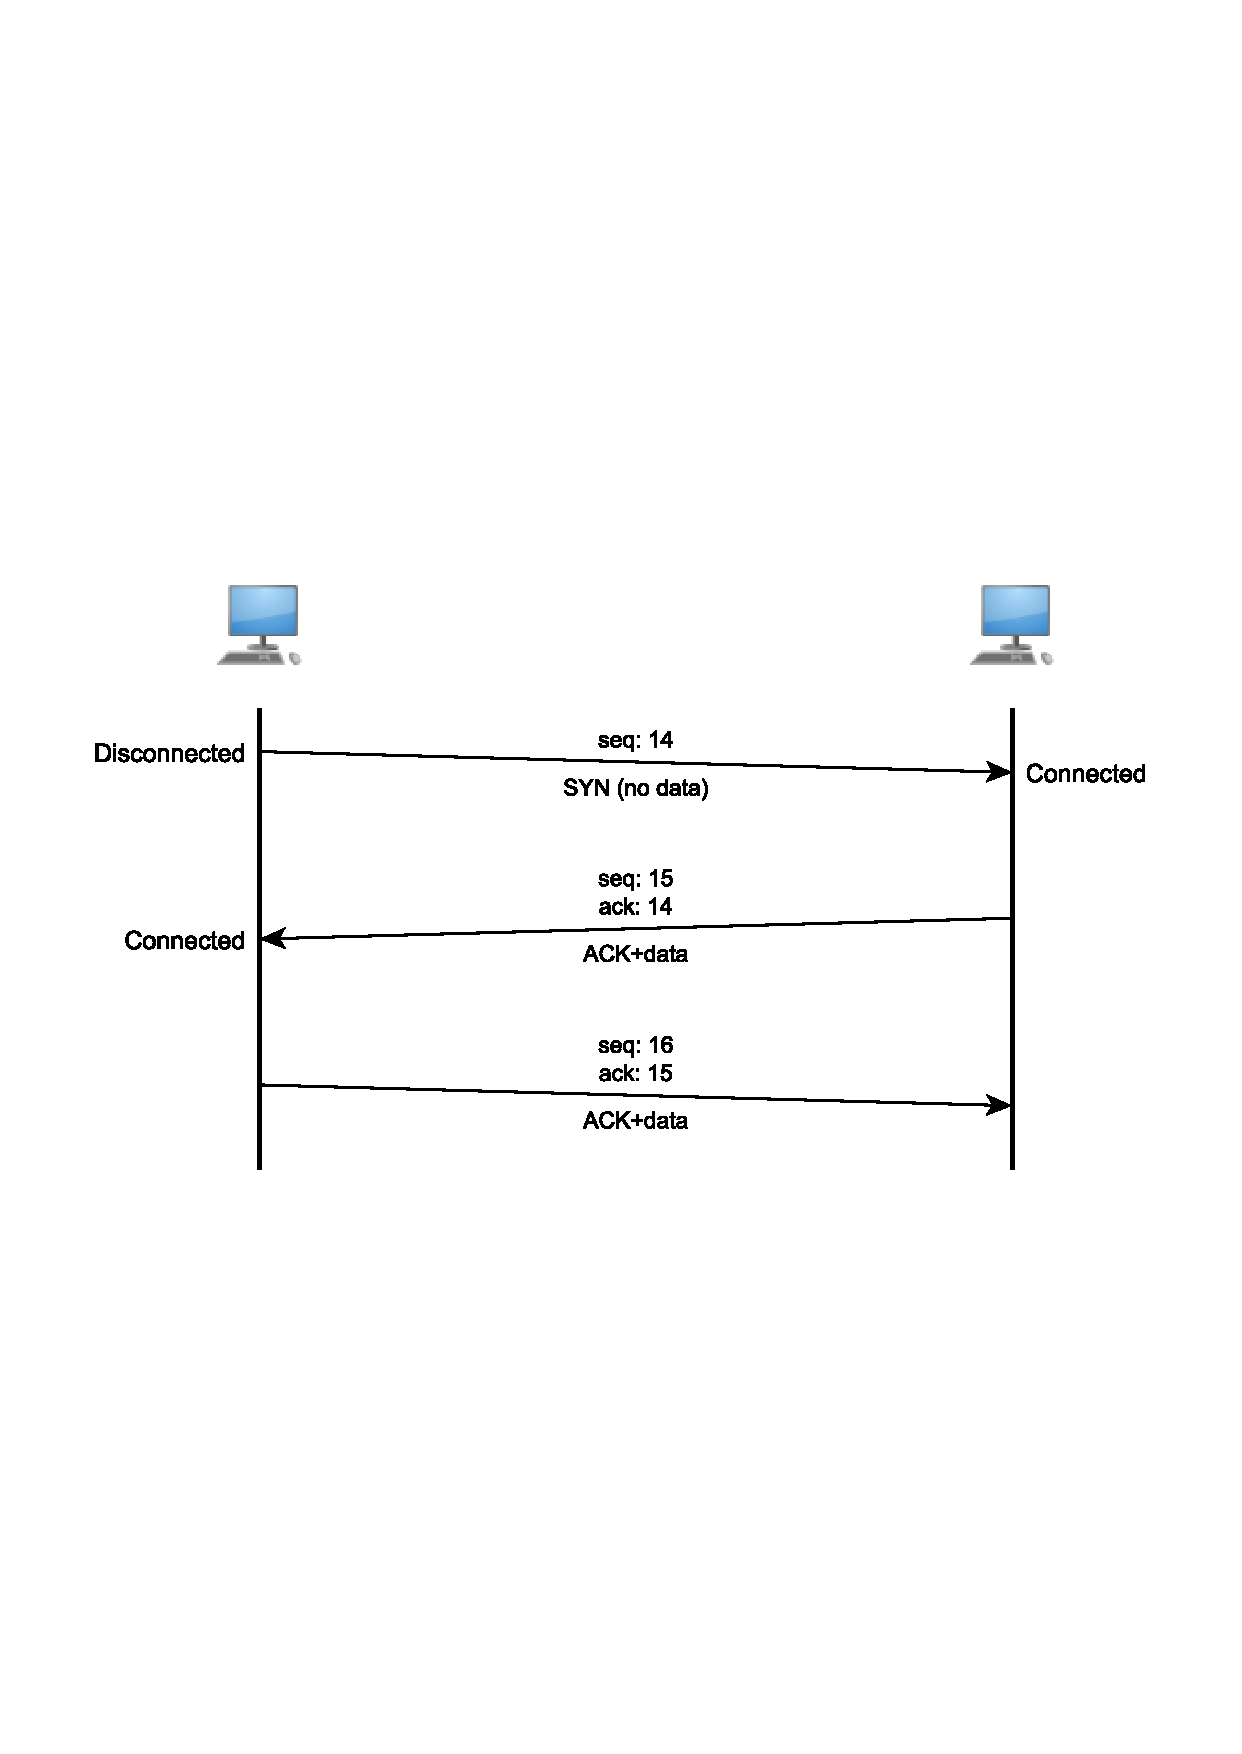
\includegraphics[scale=0.64,trim=0 264 0 266]{content/graphics/trans_syn_transfer.pdf}%trim=l b r t
 \caption{The transport layer protocol opening a connection}
 \label{fig:trans_syn_transfer}
\end{figure}

%================= OLD =================
%
%
%Consequently, protocol will contain  the properties described above, and following specifications can be formulated: The protocol should
% We wish for the protocol to
%\begin{itemize}
% \item provide reliable delivery up to a maximum number of retransmissions
% \item provide in-order delivery regardless if underlying layers
% \item have low overhead
%\end{itemize}
%
%A number of port addresses (0-19) are going to be reserved for special messages and are therefore not available for applications to use. 
%
%Refer to Table \ref{tab:trans_well_known} for a list of reserved ports and their uses.
%\begin{table}[htb]
% \centering
% \begin{tabular}{cl}
%  \textit{Port} & \textit{Description}\\
%  \midrule
%  1 & Does something?\\
%  \midrule
%  4 & Not sure what this does\\
%  \midrule
%  17 & Does something else
% \end{tabular}
% \caption{Well-known ports used by the transport layer protocol}
% \label{tab:trans_well_known}
%\end{table}
%
%
%
%\begin{table}[htb]
% \centering
% \begin{tabular}{rcccc}
%  \textit{Bits} & 0-7 & 8-15 & 16-23 & 24-255\\
%  \midrule
%   & Source port & Dest. port & Length & Data
% \end{tabular}
% \caption{Transport layer datagram format}
% \label{tab:trans_datagram_format}
%\end{table}
%
%
%
%\subsection{Operation}
%Much like the UDP\nomenclature{UDP}{User datagram protocol} this transport layer protocol provides a connectionless service, meaning packets are sent without having to first establish a connection. Also they are sent without sequence numbers, though in our case this is not a problem. This protocol will only be used on a half-duplex line, and there is no routing from one network to another: The packets can only go one way, and there is only one packet on the line at a time, thus packets cannot be ''out of order''.
%
%In this protocol, no flow or error control is incorporated.\marginnote{If needed we can implement error or flow ctrl anyway} This is mainly due to the reason that the data link layer and transport layer communicate directly, and not across networks where another protocol might provide an unreliable service (as with the IP\footnote{Internet protocol}\nomenclature{IP}{Internet protocol} which is provides \textit{best effort} delivery). With no error or flow control we save yet some more overhead space.
%
%With each application getting a different port number, the transport layer protocol being developed provides application multiplexing. That is, more than one application can use the protocol at the same time on each node. 
%
%
%%%%%%%%%%%%%%%%%%%%%%%%%%%%%%%%%%%%%%%%%%%%%%%%%%%%%%%%%%%%%%%%%%%%%%%%%%%%%%%%
% Kims ''thinking'' ^o~
%%%%%%%%%%%%%%%%%%%%%%%%%%%%%%%%%%%%%%%%%%%%%%%%%%%%%%%%%%%%%%%%%%%%%%%%%%%%%%%%
%
%error control
%multiplexing
%well known ports (for ''control'')
%datagrams (variable length, but with max.)
%
%As a low overhead is preferred, it is natural to look to the UDP\footnote{User datagram protocol}\nomenclature{UDP}{User datagram protocol}. The UDP transport layer protocol provides a connectionless service and unreliable service.
%
%Also they are sent without sequence numbers, though in our case this is not a problem. This protocol will only be used on a half-duplex line, and there is no routing from one network to another: The packets can only go one way, and there is only one packet on the line at a time, thus packets cannot be ''out of order''.
%
%
% IN:
% ----
% * Byte-array
% * Source port number       \
% * Destination port number   \_ (or do we know this already?)
%
% OUT:
% ----
% HEADER                        DATA
% 
%
% ''session''-delen er lidt ude i kulden? connection oriented transport layer protokol kan det, vi gerne vil?
%
% sekvensering
% process-process
% process ID (PID) / ''port'' number
% (de)multiplexing
% in/out queue-buffer (one for each port)
%   overflow
%   unreachable/queue non-existant
% reserved ports for system messages?
% flow control, we don't need (?)
% unrealiable sending ?
% connectionless service ?
% congestion, we dont care?
%
%
% socket address = ''data link layer''-address + port number
%
%
%variabel datal�ngde, sekvensnummer, sessionID,modtager, afsender,flag